\documentclass[11pt]{article}

% ============================================================
% main_v2.tex --- restructured draft implementing the strategic
% reorientation decided 2026-07-18/19 (see reports/paper_master_plan.md,
% "Orientation strategique du papier"). main.tex is kept intact as the
% previous draft; this file is the working narrative going forward.
%
% Narrative contract (do not drift from this without a plan update):
%   * Headline = POSITIVE: a deterministic model obtained by DELETING the
%     diffusion loop from a validated diffusion forecaster sets a new
%     state of the art -- ~9.4x the published FNO+ number at ~1/320th the
%     inference cost. Not "a negative result about diffusion".
%   * The paper's real contribution is ATTRIBUTION (level 2 of the
%     three-reading hierarchy): the gains this line of work credits to
%     generative sampling trace to representation choices (delta target,
%     regime-aware scale) that transfer unchanged to the deterministic
%     model. The non-monotone win pattern (twin wins dense+m95, m50
%     undecided) is the non-trivial empirical shape that makes this more
%     than "we ran an ablation".
%   * The procedural recommendation (always build the matched twin) is a
%     COROLLARY stated at the END of the discussion -- never the headline.
%   * Claims stay scoped: substantive findings = FloodCastBench + tested
%     architectures only; no "twin replaces FNO in general" (no-free-lunch
%     paragraph in the discussion makes this explicit).
% ============================================================

% ---------- Typography: clean, professional, journal-style ----------
\usepackage[T1]{fontenc}
\usepackage[utf8]{inputenc}
\usepackage{amsmath,amssymb,amsthm}   % load before newtxmath to avoid \Bbbk clash
\usepackage{newtxtext,newtxmath}     % Times-like serif, professional look
\usepackage[margin=1in]{geometry}
\usepackage{microtype}                % subtle spacing/kerning polish
\usepackage{setspace}
\setstretch{1.05}

% ---------- Structure & references ----------
\usepackage{booktabs}                 % clean table rules, no vertical lines
\usepackage{caption}
\usepackage{subcaption}
\usepackage{graphicx}
\usepackage[colorlinks=true,citecolor=blue!55!black,linkcolor=blue!55!black,urlcolor=blue!55!black]{hyperref}
\usepackage[round,authoryear]{natbib}
\usepackage{xcolor}
\usepackage{enumitem}
\setlist{topsep=4pt,itemsep=2pt}
\usepackage{placeins}
\usepackage{float}
\usepackage{tikz}
\usetikzlibrary{positioning,fit,arrows.meta,calc}
\definecolor{diffblue}{RGB}{0,114,178}
\definecolor{twinverm}{RGB}{213,94,0}

% ---------- Section spacing (tight, professional) ----------
\usepackage{titlesec}
\titlespacing*{\section}{0pt}{14pt}{6pt}
\titlespacing*{\subsection}{0pt}{10pt}{4pt}

% ---------- Model names (publication names, defined once) ----------
\newcommand{\ours}{\mbox{$\Delta$-Diff}}       % delta-space diffusion forecaster
\newcommand{\absdiff}{\mbox{Abs-Diff}}          % absolute-field variant (reference parametrization)
\newcommand{\twin}{\mbox{Twin}}                 % deterministic twin
\newcommand{\mfifty}{\textsc{m50}}
\newcommand{\mninetyfive}{\textsc{m95}}

% ---------- Draft-status callouts (visible in compiled PDF, removed before submission) ----------
\newcommand{\blocked}[1]{%
  \par\smallskip
  \noindent\fcolorbox{orange!70!black}{orange!8}{%
    \begin{minipage}{0.96\linewidth}
    \small\color{orange!40!black}\textbf{[PENDING --- experiment in progress]} #1
    \end{minipage}%
  }
  \smallskip\par
}
\newcommand{\readynote}[1]{%
  {\small\color{gray}\textit{#1}}
}

\title{\textbf{Subtracting the Sampler: \\
  \large A Deterministic Twin of a Diffusion Forecaster Sets the State of
  the Art \\ for Flood Prediction under Sparse Observation}}
\author{Wissam Abdelwahed}
\date{\today}

\begin{document}
\maketitle

\begin{abstract}
\noindent
Conditional diffusion models are increasingly applied to spatiotemporal
forecasting under partial observation, on the premise that a generative
model's sampling distribution provides value a deterministic model cannot.
We put that premise under the most direct test we know of. We first build
the strongest diffusion forecaster we can for autoregressive flood
prediction on FloodCastBench: identifying and correcting a structural
failure of the reference parametrization (diffusing the \emph{absolute}
water-depth field at fine cadence, where the per-step physical change is
450--490$\times$ smaller than the field's amplitude), our delta-space,
regime-aware model outperforms the strongest published neural-operator
baseline (FNO+) on all five reported metrics under full observation. We
then \emph{delete its diffusion loop}: the resulting parameter- and
protocol-matched deterministic twin --- identical weights, training, and
inputs; a single forward pass in place of 320 network evaluations --- is
better still, reaching a relative RMSE $\sim$9.4$\times$ below the
published state of the art at $\sim$1/320th the diffusion model's
inference cost. Across observation regimes the controlled comparison is
non-monotone in an informative way: the twin wins decisively both under
full observation and under extreme (95\%) sparsity, with only the
intermediate regime statistically undecided across seeds --- sparsity
level alone does not predict a generative advantage. A preliminary
zero-shot cross-region transfer (Australia-trained models evaluated
unchanged on the UK event) preserves the pattern against the benchmark's
published transfer results. On uncertainty, a deep ensemble of twins is
never worse calibrated than the diffusion model's own scenario ensemble.
Taken together, the gains this line of work attributes to generative
sampling trace, on this benchmark, to \emph{representation choices ---
delta-space targets and regime-aware scaling --- that transfer unchanged
to a deterministic model}; we propose the matched-twin control as standard
practice before attributing forecasting gains to a generative mechanism.
\end{abstract}

\begin{center}
\readynote{Working draft (v2 narrative) compiled \today\ --- boxes marked
PENDING depend on experiments still running; every number outside a
PENDING box is final unless its caption states otherwise.}
\end{center}

% ============================================================
\section{Introduction}
\label{sec:intro}

Flood forecasting at deployment time is a sparse-observation problem: a
real sensor network samples the water surface at a small fraction of the
grid cells a hydraulic model would need, and any forecaster must
reconstruct-and-predict from that partial view. A growing line of work
answers this with conditional diffusion models
\citep{diffsparse2025,jamesstations2025,jamesocean2025,phyda2025},
importing an approach validated in genuinely stochastic domains ---
medium-range weather above the deterministic predictability horizon
\citep{gencast2024} --- on the premise that a generative model's scenario
distribution captures something a deterministic model cannot.

This paper reports what happened when we subjected that premise to the
most direct test we know of. We first built the strongest diffusion
forecaster we could on a public flood benchmark
\citep{floodcastbench2025}: after diagnosing why the reference
parametrization fails at fine temporal cadence (\S\ref{sec:mechanism}),
our corrected model, \ours{}, beats the benchmark's strongest published
baseline (FNO+) on all five reported metrics (\S\ref{sec:vsfnoplus}).
We then performed the simplest possible intervention: \emph{we deleted
the diffusion loop}. The resulting deterministic twin --- the same
network, weights-for-weights, evaluated once with the noise input and
diffusion time index fixed to zero instead of sampled over 40 denoising
steps $\times$ 8 scenarios --- is not merely competitive. It is the best
model we measure on the benchmark: $\sim$9.4$\times$ below the published
state-of-the-art relative RMSE under full observation, at
$\sim$1/320th the diffusion model's inference cost, and decisively ahead
under extreme sparsity as well (\S\ref{sec:twinresults}).

Two aspects of this outcome are not what either pre-registered
expectation predicted. First, the pattern across observation regimes is
\textbf{non-monotone}: the twin dominates at both ends of the
observability spectrum (fully observed, and 95\%-masked), while the
intermediate 50\%-masked regime is genuinely undecided --- the sign of
the difference flips across training seeds and across every metric we
compute. A simple ``deterministic always wins on a deterministic
target'' story would predict uniform dominance; the data refuse it.
Second, the entire advantage the generative line of work would attribute
to sampling turns out to be carried by \emph{representation choices} ---
a delta-space target and a regime-aware scale (\S\ref{sec:regime}) ---
that transfer to the deterministic model unchanged. The generative
mechanism itself, once these choices are held fixed, never shows a
seed-consistent advantage anywhere we measure.

These results support three readings, in increasing order of scope.
Narrowly: on FloodCastBench-like tasks, the diffusion loop is a cost, not
a benefit, and practitioners building on this line of work should know
that. At the level we consider the paper's real contribution:
\textbf{attribution} --- gains in this literature credited to generative
sampling can originate entirely in parametrization, and only a
parameter-matched deterministic control can tell the difference; we
supply the first such control for this task family and the specific,
non-obvious pattern it reveals. Broadly, and more tentatively: flood
forecasting against a deterministic simulator sits below the
predictability horizon that justified generative forecasting in weather
--- the ``uncertainty'' a scenario ensemble captures here is
reconstruction ambiguity, not chaotic divergence
(\S\ref{sec:calibmeaning}) --- and our calibration results
(\S\ref{sec:calibration}) show a deep ensemble of deterministic twins
quantifies that ambiguity at least as well as the diffusion ensemble
does.

\paragraph{Contributions.}
\begin{enumerate}
  \item \textbf{A new state of the art on FloodCastBench}, twice over:
    \ours{} beats the published FNO+ results on all five metrics under
    full observation, and its deterministic twin improves on \ours{} by a
    further $\sim$3.7$\times$ at $\sim$1/320th the inference cost
    (\S\ref{sec:vsfnoplus}, \S\ref{sec:twinresults}).
  \item \textbf{The first parameter- and protocol-matched
    deterministic--generative control} for autoregressive flood
    forecasting under sparsity, and the non-monotone advantage pattern it
    reveals (\S\ref{sec:twinresults}), robust across six metrics and to a
    checkpoint-convergence audit.
  \item \textbf{A quantified failure mechanism (stated as a tested
    hypothesis)} for absolute-field diffusion at fine cadence --- a
    450--490$\times$ target-scale mismatch measured on two independent
    events --- with a pre-registered dose--response design to settle it
    (\S\ref{sec:mechanism}).
  \item \textbf{A calibration audit under a deterministic simulator},
    comparing the diffusion ensemble against the standard deep-ensemble
    baseline it should be, but is not, compared against in this
    literature (\S\ref{sec:calibration}).
  \item \textbf{Methodological guardrails} we expect to outlive the
    specific numbers: the single-draw-vs-mean statistical trap
    (\S\ref{sec:twin}), and the matched-twin protocol itself as a
    corollary recommendation (\S\ref{sec:discussion}).
\end{enumerate}

\blocked{Two additions will strengthen this introduction before freeze,
without changing its claims: (i) the dose--response result
(\S\ref{sec:mechanism}) will upgrade contribution 3 from ``tested
hypothesis'' to either ``demonstrated mechanism'' or an honest
retraction; (ii) the cross-region transfer section
(\S\ref{sec:zeroshot}) currently rests on a 3-window UK test split ---
the Pakistan$\to$Mozambique replication (training paused at the time of
writing, \S\ref{sec:zeroshot}) will either consolidate or qualify the
transfer claim.}

% ============================================================
\section{Related Work}
\label{sec:related}

Diffusion-based reconstruction under sparse observation has been explored
along two largely disjoint lines. The first targets tidal and coastal
flood forecasting directly: \citet{diffsparse2025} diffuse a coastal
water-level field under 0/50/95\% sparsity and report up to 62\% error
reduction over baseline methods, but do not include a parameter-matched
deterministic control, do not diagnose a failure mechanism for their own
parametrization, and do not evaluate the calibration of their generated
ensembles. \citet{spatiallyawarediffusion2024} reconstruct static PDE
fields from sparse sensors with a hybrid conditioning scheme close to our
spatial encoder, and --- notably --- independently conclude that a
deterministic model wins in the noise-free regime while diffusion only
helps once observation noise is introduced; we extend this finding to the
\emph{autoregressive}, real-benchmark setting and quantify a concrete
parametrization-level mechanism behind it (\S\ref{sec:mechanism}). A second
line applies conditional diffusion to data assimilation at
national-to-global scale for weather and ocean state
\citep{jamesstations2025,jamesocean2025,phyda2025} --- an active area, but
none of this work runs a matched deterministic control, and none targets
pluvial or fluvial flood forecasting. \citet{sf2bench2025} provide real
river-gauge time series but no spatial field reconstruction, making it
complementary rather than substitutable. \citet{floodcastbench2025} is, to
our knowledge, the only public benchmark combining high-fidelity flood
fields, physical forcings (terrain elevation, rainfall), and
neural-operator baselines (U-Net, FNO, FNO+) at the resolution and cadence
used here, and is the benchmark we build on. Its strongest baseline, FNO+,
descends from the Fourier Neural Operator \citep{li2021fno}, whose global
spectral mixing and resolution-invariance were designed for, and validated
on, globally smooth PDE fields (Navier--Stokes, Darcy flow) --- a design
point whose consequences for sharp-fronted flood fields we return to in
the discussion (\S\ref{sec:discussion}).

No existing work, to our knowledge, runs a parameter- and protocol-matched
deterministic-vs-generative comparison for autoregressive flood forecasting
under sparse observation. This is the gap we address.

% ============================================================
\section{Problem Setup}
\label{sec:setup}

\subsection{Task}
We consider the task of forecasting the spatiotemporal evolution of a
flood --- a dense field of water depth over a fixed spatial grid --- from a
\emph{partially observed} current state. At full observation density
(``dense''), the current water-depth field is known everywhere; under
sparsity, only a subset of grid cells (standing in for a real sensor
network) is observed at each time step, with the rest masked. Forecasts
are autoregressive: models roll forward twelve 300-second steps,
re-consuming their own prediction as the next step's context.

\subsection{Benchmark}
We use FloodCastBench's high-fidelity Australia event at 60\,m resolution
\citep{floodcastbench2025}: 2{,}881 water-depth frames at 300\,s cadence on
a $536\times536$ grid, paired with a static digital elevation model (DEM)
and time-varying rainfall at 1800\,s resolution (each rainfall frame
repeated across the six 300\,s steps it covers, matching the benchmark's
own data-generation convention). The United Kingdom 2015 event (60\,m,
$85\times137$ grid, 865 frames) additionally serves as a zero-shot
transfer target (\S\ref{sec:zeroshot}): Australia-trained models are
evaluated on it with frozen weights and frozen normalization, mirroring
the benchmark's own cross-regional transfer protocol.
\blocked{A full in-domain second-event study (training and evaluating
both models on the UK event across all three sparsity regimes, 3 seeds)
is queued; it is deliberately sequenced \emph{after} per-window error
logging lands in the evaluator, so that its evaluations directly support
the pre-registered window$\times$seed paired significance test
(\S\ref{sec:protocol}) without being re-run. Until then, all in-domain
numbers refer to the Australia event.}

\subsection{Sparsity protocol}
We evaluate three observation regimes: \textbf{dense} (100\% observed),
\textbf{\mfifty} (50\% of cells unobserved), and \textbf{\mninetyfive}
(95\% unobserved). Masks are random i.i.d., drawn from a fixed seeded bank
reused across all models so that every model sees identical observation
patterns. To test whether conclusions drawn under random masking
generalize to \emph{realistic} sensor deployments, we additionally
evaluate two structured mask families never seen during training: a
\textbf{gauge} proxy (sensors concentrated where water is present
initially, approximating river-gauge placement) and a \textbf{cluster}
mask (spatially contiguous unobserved regions, approximating a coverage
gap) --- \S\ref{sec:masks}.

\subsection{What ``calibration'' can mean here}
\label{sec:calibmeaning}
FloodCastBench's ground truth is generated by a single deterministic
hydraulic simulation per event --- there is no ensemble of physical
realizations to calibrate against. The uncertainty a generative model's
scenario spread can meaningfully quantify here is therefore the
\emph{ambiguity of reconstruction under partial observation} (how many
distinct complete fields are consistent with a given sparse observation),
not aleatoric physical uncertainty. We evaluate calibration under this
reading throughout, and state it explicitly rather than let the term imply
more than the data can support.

% ============================================================
\section{Methods}
\label{sec:methods}

\subsection{The controlled pair: a diffusion forecaster and its deterministic twin}
\label{sec:twin}
Our diffusion forecaster --- \ours{}, named for the delta-space
parametrization introduced in \S\ref{sec:mechanism} --- predicts, at each
step, the \emph{change} in the water-depth field conditioned on the sparse
observation history, terrain, and rainfall. To isolate whether a
generative model's value comes from its generative mechanism specifically
--- as opposed to its architecture, training budget, or input context ---
we construct a \textbf{deterministic twin} (\twin{}): a model sharing
\ours{}'s exact encoders, backbone, parameter count (verified weight-for-weight,
not approximately), training budget, checkpoint-selection rule, and
training curriculum, with the diffusion loop replaced by a single
deterministic forward pass (the noise input fixed to zero and the
diffusion time index to zero). This is, to our knowledge, the first such
matched control for autoregressive flood forecasting under sparsity.
Figure~\ref{fig:pair} summarizes the shared architecture and the single
point at which the two models differ.

\begin{figure}[H]
\centering
\resizebox{\linewidth}{!}{%
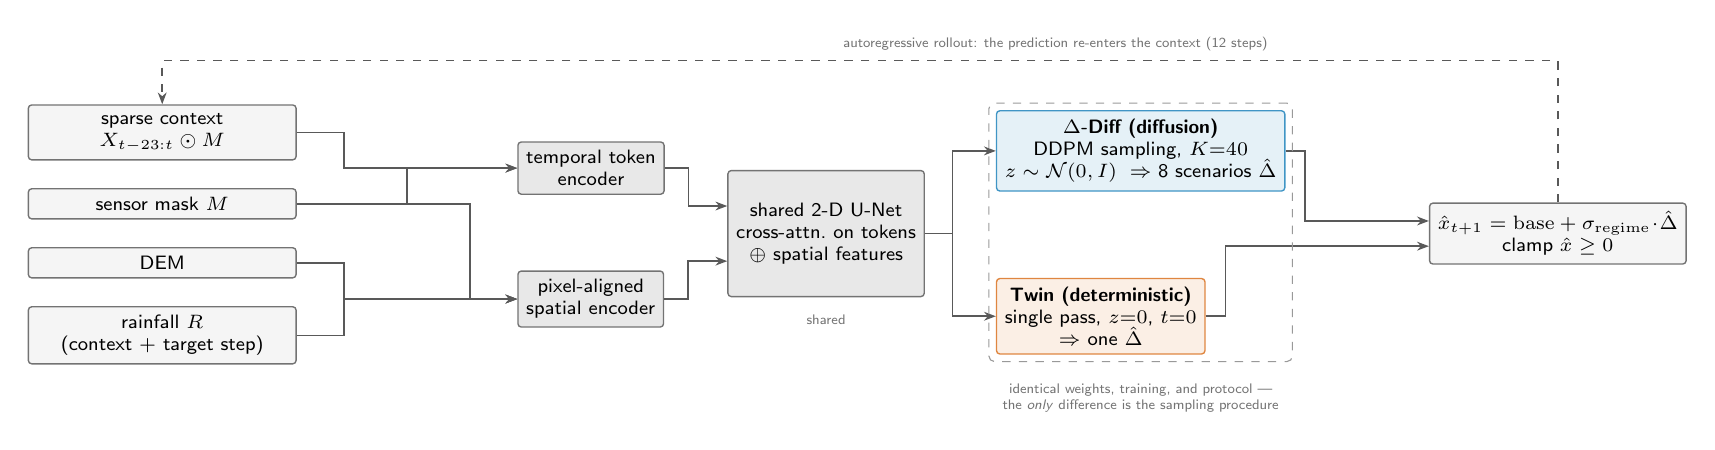
\begin{tikzpicture}[
  font=\sffamily\scriptsize,
  node distance=3.5mm and 6mm,
  box/.style={draw=black!55, rounded corners=1.2pt, align=center, inner sep=3pt, fill=black!4, line width=0.5pt},
  enc/.style={box, fill=black!9},
  headv/.style={box, fill=diffblue!10, draw=diffblue!75},
  headt/.style={box, fill=twinverm!10, draw=twinverm!75},
  arr/.style={-{Stealth[length=1.5mm]}, black!65, line width=0.55pt},
  lab/.style={font=\sffamily\tiny, black!55, align=center},
]
% ---- inputs: forced to a common width so their .east edges align exactly ----
\node[box, minimum width=34mm] (xin) {sparse context\\ $X_{t-23:t}\odot M$};
\node[box, minimum width=34mm, below=of xin] (min) {sensor mask $M$};
\node[box, minimum width=34mm, below=of min] (dem) {DEM};
\node[box, minimum width=34mm, below=of dem] (rain) {rainfall $R$\\ (context $+$ target step)};
% ---- shared encoders ----
\coordinate (encx) at ($(rain.east)+(28mm,0)$);
\coordinate (tency) at ($(xin.east)!0.5!(min.east)$);
\coordinate (sency) at ($(dem.east)!0.5!(rain.east)$);
\node[enc, anchor=west] (tenc) at (encx |- tency) {temporal token\\ encoder};
\node[enc, anchor=west] (senc) at (encx |- sency) {pixel-aligned\\ spatial encoder};
% ---- shared U-Net ----
\coordinate (unety) at ($(tenc.east)!0.5!(senc.east)$);
\coordinate (unetx) at ($(senc.east)+(8mm,0)$);
\node[enc, anchor=west, minimum height=16mm] (unet) at (unetx |- unety) {shared 2-D U-Net\\ cross-attn.\ on tokens\\ $\oplus$ spatial features};
% ---- two inference heads ----
\node[headv, anchor=west] (v2) at ($(unet.east)+(9mm,10.5mm)$) {\textbf{\ours{} (diffusion)}\\ DDPM sampling, $K{=}40$\\ $z\sim\mathcal N(0,I)\;\Rightarrow\;$8 scenarios $\hat\Delta$};
\node[headt, anchor=west] (tw) at ($(unet.east)+(9mm,-10.5mm)$) {\textbf{\twin{} (deterministic)}\\ single pass, $z{=}0$, $t{=}0$\\ $\Rightarrow$ one $\hat\Delta$};
% ---- reconstruction ----
\node[box, anchor=west] (rec) at ($(unet.east)+(64mm,0)$) {$\hat x_{t+1}=\mathrm{base}+\sigma_{\mathrm{regime}}\!\cdot\!\hat\Delta$\\ clamp $\hat x\ge 0$};
% ---- arrows: all orthogonal ----
\draw[arr] (xin.east) -- ++(6mm,0) |- (tenc.west);
\draw[arr] (dem.east) -- ++(6mm,0) |- (senc.west);
\draw[arr] (rain.east) -- ++(6mm,0) |- (senc.west);
\draw[arr] (min.east) -- ++(14mm,0) |- (tenc.west);
\draw[arr] (min.east) -- ++(22mm,0) |- (senc.west);
\draw[arr] (tenc.east) -- ++(3mm,0) |- ($(unet.west)+(0,3.5mm)$);
\draw[arr] (senc.east) -- ++(3mm,0) |- ($(unet.west)+(0,-3.5mm)$);
\draw[arr] (unet.east) -- ++(3.5mm,0) |- (v2.west);
\draw[arr] (unet.east) -- ++(3.5mm,0) |- (tw.west);
\draw[arr] (v2.east) -- ++(2.5mm,0) |- ($(rec.west)+(0,1.6mm)$);
\draw[arr] (tw.east) -- ++(2.5mm,0) |- ($(rec.west)+(0,-1.6mm)$);
% autoregressive feedback (orthogonal)
\draw[arr, dashed] (rec.north) -- ++(0,18mm) -| node[pos=0.18, above, lab] {autoregressive rollout: the prediction re-enters the context (12 steps)} (xin.north);
% shared-vs-differs annotation
\node[draw=black!40, dashed, rounded corners=2pt, fit=(v2)(tw), inner sep=2.5pt] (differ) {};
\node[lab, below=1.5mm of differ.south] {identical weights, training, and protocol ---\\ the \emph{only} difference is the sampling procedure};
\node[lab, below=1mm of unet.south] {shared};
\end{tikzpicture}%
}
\caption{The controlled pair. Both models share every component --- inputs,
temporal token encoder, pixel-aligned spatial encoder, U-Net backbone,
delta-space target with per-regime scale $\sigma_{\mathrm{regime}}$
(\S\ref{sec:regime}), training protocol, and autoregressive rollout.
The diffusion forecaster (\ours{}) draws $K{=}40$ denoising steps from
Gaussian noise to produce 8 scenarios; the deterministic twin (\twin{})
evaluates the same network once with the noise input and diffusion time
index fixed to zero. Any performance difference between the two is
therefore attributable to the generative mechanism itself.}
\label{fig:pair}
\end{figure}

\paragraph{A statistical trap in comparing the two, and why it matters.}
For any predictive distribution,
\begin{equation}
\mathbb{E}\big[(x_{\text{sample}} - x_{\text{truth}})^2\big]
  = \mathrm{Var}(\text{posterior}) + \mathbb{E}\big[(\bar{x} - x_{\text{truth}})^2\big]
  \;\geq\; \mathbb{E}\big[(\bar{x} - x_{\text{truth}})^2\big],
\end{equation}
so a single draw from a generative model carries strictly more expected
squared error than the predictive mean, purely as a property of variance,
regardless of model quality. A deterministic regressor targets the mean
directly. Comparing a single generative draw to a deterministic output on
RMSE is therefore \textbf{mathematically biased toward the deterministic
model by construction}. We encountered this bias affecting our own model
selection during development (an internal validation metric used a single
rollout draw) and corrected for it: every decision-relevant comparison in
this paper scores \ours{} by the \emph{mean of its 8 scenarios}. We flag
this explicitly as a generic trap for any future
deterministic-vs-generative comparison in this literature.

\subsection{Why does the absolute field fail at fine cadence? A scale-mismatch hypothesis}
\label{sec:mechanism}
A first variant of our forecaster --- \absdiff{}, which follows the
reference parametrization of \citet{diffsparse2025} and diffuses the
\emph{absolute} water-depth field --- fails catastrophically at the
benchmark's native 300-second cadence: in the dense regime it is
$\sim$560$\times$ worse than trivial persistence (predicting no change at
all). The failure is not an implementation defect, and it is not a
property of diffusion itself: the delta-space model built on the same
skeleton works (\S\ref{sec:paramresults}). What distinguishes the two is
the \emph{scale of the generative target}. The true physical signal
between two consecutive frames is tiny relative to the field's own
amplitude: writing $\sigma_\Delta$ for the standard deviation of per-step
changes and $\sigma_{\text{field}}$ for that of the wet-pixel depths, we
measure, directly from the raw data of two independent events,
\begin{equation}
\sigma_{\text{field}} / \sigma_\Delta \;\approx\; 488 \text{ (Australia)}, \qquad 425 \text{ (UK)}
\end{equation}
(Figure~\ref{fig:mechanism}). Our working hypothesis is a
\textbf{sampling-noise floor}: if a sampler's residual error scales with
the amplitude of its generative target with some model-specific constant
$c$, then beating persistence requires $c < \sigma_\Delta /
\sigma_{\text{field}} \approx 1/450$ in absolute space --- far below what
practical samplers achieve --- but only $c < 1$ in delta space, which is
trivially met. We state this as a hypothesis rather than a demonstrated
mechanism: the evidence so far is two events, both with a high ratio
\emph{and} a failure, from the same benchmark family --- consistent with
the hypothesis, but not yet a dose--response relationship.

The data-only groundwork for the decisive test is already in place:
Figure~\ref{fig:doseresponse} shows how the measured ratio falls as the
effective time step $\Delta t$ grows (subsampling the existing frames),
from $\sim$478 at the native 300\,s to $\sim$21 at 7200\,s (Australia;
UK behaves identically). Because $\sigma_\Delta$ grows near-linearly with
$\Delta t$ over this range (smooth advective flow, no decorrelation), the
achievable span covers a factor $\sim$23 of the ratio but cannot reach
parity (ratio $\approx 1$) by subsampling alone --- so the pre-registered
prediction is the \emph{monotone closing} of the absolute-vs-delta gap
over the achievable range, not full parity.

\blocked{The dose--response training runs themselves are the pending
piece: one fixed skeleton (\ours{}'s), a single crossed factor
\{$\Delta t \in$ 300, 900, 1800, 7200\,s\} $\times$ \{target: absolute,
delta\} --- 8 short single-step training runs in the dense regime (no
rollout confounds), seed 42, screening-labeled. The hypothesis predicts
the absolute-arm-to-delta-arm error ratio shrinks monotonically as the
scale ratio falls. There is no universal threshold to find --- the
crossing point depends on the sampler's own constant $c$ --- but
monotonicity tests the mechanism, and the empirical crossing point for
this architecture is a citable, explicitly non-universal deliverable.
Outcome contract: monotone $\Rightarrow$ \S\ref{sec:mechanism} upgrades
from hypothesis to demonstrated mechanism and
Figure~\ref{fig:doseresponse} gains the two training arms; non-monotone
$\Rightarrow$ the mechanism claim is retracted to an empirical
observation and the contribution list is edited accordingly. An internal
hint is already consistent with the hypothesis: the
\absdiff{}-vs-\ours{} gap compresses exactly where the delta target's
effective scale grows (from $970\times$ dense to $1.9\times$ at
\mninetyfive{}, where masked pixels make the delta target field-scaled),
though that comparison is confounded with sparsity itself --- hence the
clean test.}

\begin{figure}[H]
  \centering
  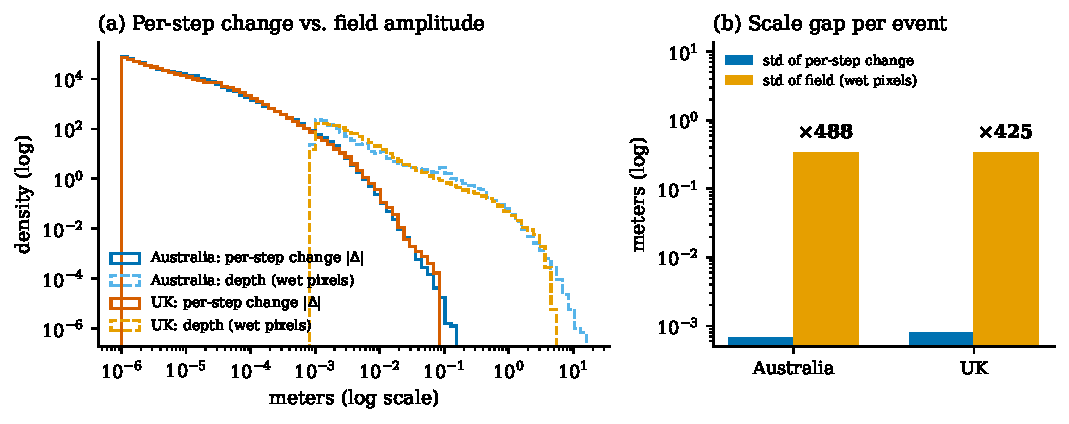
\includegraphics[width=0.92\linewidth]{figures/f2_mechanism.pdf}
  \caption{The scale mismatch behind the absolute-field failure
  hypothesis, measured from raw training data of two independent flood
  events. (a) The distribution of per-step changes $|\Delta|$ sits two to
  three orders of magnitude below the wet-pixel depth distribution.
  (b) The resulting scale gap ($\sim$488$\times$ Australia,
  $\sim$425$\times$ UK) is, under the sampling-noise-floor hypothesis, a
  lower bound on the relative sampling accuracy an absolute-field
  diffusion model would need just to match persistence.}
  \label{fig:mechanism}
\end{figure}

\begin{figure}[H]
  \centering
  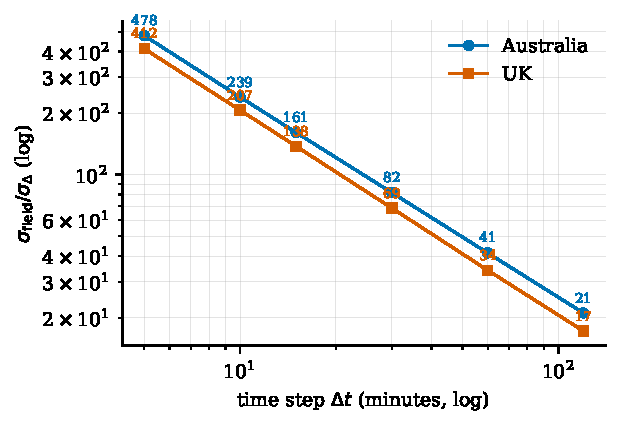
\includegraphics[width=0.7\linewidth]{figures/f2b_dose_response_ratio.pdf}
  \caption{Dose--response groundwork (data-only, no model): the measured
  scale ratio $\sigma_{\text{field}}/\sigma_\Delta$ as a function of the
  effective time step $\Delta t$, obtained by subsampling the existing
  frame sequences. $\sigma_\Delta$ grows near-linearly in $\Delta t$ on
  both events, so the ratio falls as $\sim 1/\Delta t$, spanning
  478$\to$21 (Australia) and 412$\to$17 (UK). The four marked $\Delta t$
  values are the pre-registered training points for the pending
  dose--response experiment (see box above); the parity region (ratio
  $\approx$1) is unreachable by subsampling alone, which bounds what the
  experiment can and cannot show and is stated as such.}
  \label{fig:doseresponse}
\end{figure}

\subsection{Per-regime scale under partial observation}
\label{sec:regime}
Under sparsity, a further complication arises: at an observed pixel the
natural target scale is the change from its last known value
($\sigma_\Delta$); at a masked pixel the target is the change from a
training-mean fill, whose scale is closer to $\sigma_{\text{field}}$. A
single global normalization for both either drowns the observed-pixel
signal or destabilizes the masked-pixel one --- an instability we
encountered directly during development (training diverged with
non-finite losses under exactly this defect, then was corrected and
regression-tested). \ours{} therefore uses a \textbf{per-pixel,
regime-aware scale} $\sigma_{\mathrm{regime}}$, resolved at each pixel
from its observed/masked status at the current step.

\subsection{Architecture summary}
\absdiff{} uses the reference architecture of \citet{diffsparse2025} with
a 12-frame input context. \ours{} widens the temporal token encoder, adds
a pixel-aligned spatial conditioning pathway, and extends the context to
24 frames. Because the longer context is a potential confounder, we ablate
it: a \ours{} retrained at the \emph{same} 12-frame context as \absdiff{}
retains essentially the entire advantage (dense $970\times$, \mfifty{}
$3.9\times$, \mninetyfive{} $1.9\times$ over \absdiff{} on a screening
evaluation) --- the gain is architectural and parametric, not an artifact
of seeing more history. \blocked{The context ablation is currently
single-seed; it will be confirmed on two further seeds before this draft
is frozen.}

% ============================================================
\section{Evaluation Protocol}
\label{sec:protocol}

All headline numbers use the benchmark's full test protocol: the test
split of the Australia event ($13$ complete evaluation windows of 24
context $+$ 12 prediction frames), tiled rollout over overlapping
$64\times64$ patches (stride 32) with Hann-blended seams, and, for
\ours{}, 8 sampled scenarios per prediction scored by their mean
(\S\ref{sec:twin}). Evaluation masks come from a fixed seeded bank shared
identically across all models and seeds. Two persistence references
anchor every table: \emph{oracle} persistence (no change, computed from
the true dense field --- the harder bar) and \emph{sparse} persistence
(no change, computed from the masked observation only). Every headline
comparison reports mean $\pm$ std over 3 training seeds (42/7/123); no
single-seed number appears without an explicit screening label.

\paragraph{Convergence audit.} Midway through the study, an audit found
that sparse-regime checkpoints of \emph{both} models were under-trained
under the original budget (retraining improved \ours{}'s internal
selection metric by 16--37\%). Every sparse-regime number in this paper
therefore comes from checkpoints retrained under an extended budget
(early-stopping patience 120 epochs, cap 600), and the central
comparison's verdict was re-derived from scratch on the corrected
checkpoints --- with, as reported in \S\ref{sec:twinresults}, no change
in conclusion.

\paragraph{Significance.} The current check is a seed-paired sign test:
whether the per-seed difference (\ours{} $-$ \twin{}) keeps one sign
across all 3 seeds ($n{=}3$ paired differences). This is sufficient to
distinguish consistent from inconsistent directions but is not a
calibrated $p$-value. \blocked{Per-window error logging is being added to
the evaluator, enabling the pre-registered window$\times$seed paired test
($13$ windows $\times$ 3 seeds, $n{=}39$; Wilcoxon signed-rank and a
paired bootstrap). It is deliberately sequenced \emph{before} the UK
in-domain runs so those evaluations are produced once, with the right
logging, rather than re-run. Headline tables will gain confidence
intervals when it lands; the sign-test column remains as the
coarse-grained summary.}

% ============================================================
\section{Results}
\label{sec:results}

\subsection{A new state of the art under full observation}
\label{sec:vsfnoplus}
A natural objection to any claim of beating a published baseline is that
the comparison might reflect an imperfect reproduction. Our own FNO+
reproduction indeed sits $1.66\times$ above the published relative RMSE
--- a gap we attribute to undisclosed preprocessing details after
eliminating implementation error. We therefore compare against the
\emph{published} FNO+ numbers directly \citep{floodcastbench2025},
sidestepping the reproduction question entirely
(Table~\ref{tab:vsfnoplus}). \ours{} outperforms on all five reported
metrics.

\begin{table}[H]
\centering
\caption{\ours{} under full observation (mean $\pm$ std over 3 training
seeds) versus the \emph{published} FNO+ results on the same benchmark
split. Arrows give the direction of improvement; \textbf{bold} marks the
better value per row. Full test protocol (13/13 windows).}
\label{tab:vsfnoplus}
\begin{tabular}{lrr}
\toprule
Metric & FNO+ (published) & \ours{} (ours) \\
\midrule
Relative RMSE $\downarrow$ & 0.003941 & $\mathbf{0.001558 \pm 0.000836}$ \\
NSE $\uparrow$              & 0.999979 & $\mathbf{0.999996 \pm 0.000004}$ \\
Pearson $r$ $\uparrow$      & 0.999990 & $\mathbf{0.999999 \pm 0.000001}$ \\
CSI@0.001\,m $\uparrow$     & 0.939638 & $\mathbf{0.985861 \pm 0.003884}$ \\
CSI@0.01\,m $\uparrow$      & 0.984588 & $\mathbf{0.999063 \pm 0.000416}$ \\
\bottomrule
\end{tabular}
\end{table}

\paragraph{The stronger result is the twin.} \ours{}'s deterministic twin
--- the same network with the sampling loop deleted --- reaches a dense
relative RMSE of $0.000417 \pm 0.000039$ (Table~\ref{tab:twinresults}):
$\sim$\textbf{9.4$\times$ below the published state of the art}, from a
\emph{single} forward pass per prediction where \ours{} spends 40
denoising steps $\times$ 8 scenarios ($\sim$1/320th the network
evaluations). The best model on this benchmark, by a wide margin, is a
deterministic one obtained by subtracting the generative mechanism from a
diffusion model --- a result invisible without the matched-twin control.

\paragraph{Protocol differences, stated plainly.} These comparisons are
against published numbers produced under FNO+'s own protocol: a
single-shot prediction of 19 steps in one forward pass from true initial
conditions, scored deterministically. Our models are autoregressive
(errors compound across 12 steps, a structurally harder inference
setting), and \ours{} is scored by its 8-scenario mean while \twin{}, like
FNO+, produces a single deterministic output. We consider the comparison
conservative in our disfavor on the autoregressive axis, and note that the
\twin{}-vs-FNO+ comparison in particular matches deterministic output to
deterministic output; nevertheless the protocols are not identical, and we
state this rather than leave it to be discovered.

Both results hold even though \ours{}'s input context (24 frames) exceeds
FNO+'s (a single observed frame --- the official architecture broadcasts
one observation across its input time positions rather than consuming a
real history). We tested the obvious rejoinder directly rather than argue
it away: retraining FNO+ \emph{with} the same 24-frame context makes it
\textbf{worse}, not better (relative RMSE $0.007529\pm0.000328$ vs.\ its
own $0.006550\pm0.000135$ baseline, confirmed over 3 seeds). Additional
input history alone therefore does not explain the margin.

\subsection{Parametrization dominates; context length does not explain it}
\label{sec:paramresults}
Figure~\ref{fig:sparsity} compares the model family across observation
regimes. Two facts stand out. First, the delta-space parametrization is
worth up to three orders of magnitude: \absdiff{} sits at or above the
persistence level everywhere, while every delta-space model is far below
it --- as the scale-mismatch hypothesis of \S\ref{sec:mechanism} predicts.
Second, the short-context ablation confirms the advantage is not driven by
input history (\S\ref{sec:vsfnoplus} showed the same for the baseline).

\begin{figure}[H]
  \centering
  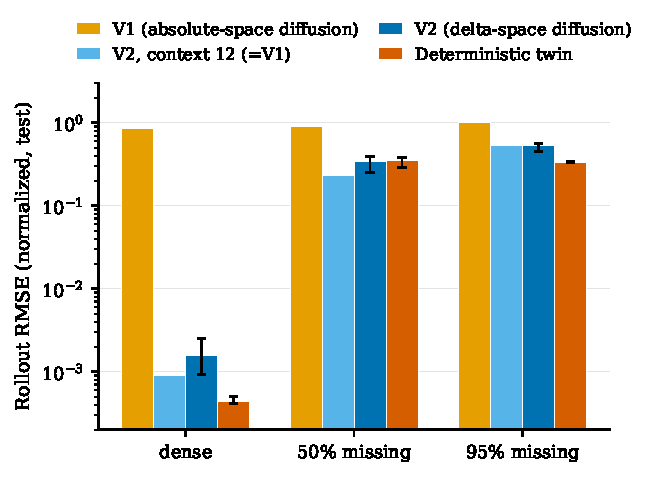
\includegraphics[width=0.78\linewidth]{figures/f3_performance_sparsity.pdf}
  \caption{Rollout RMSE (normalized, test set, log scale) across
  observation regimes. \absdiff{} and the short-context \ours{}: single
  seed (screening); \ours{} and \twin{}: mean of 3 seeds, error bars span
  the seed range, corrected checkpoints (\S\ref{sec:protocol}).}
  \label{fig:sparsity}
\end{figure}

\subsection{Diffusion vs.\ its deterministic twin: the central comparison}
\label{sec:twinresults}

\begin{figure}[H]
  \centering
  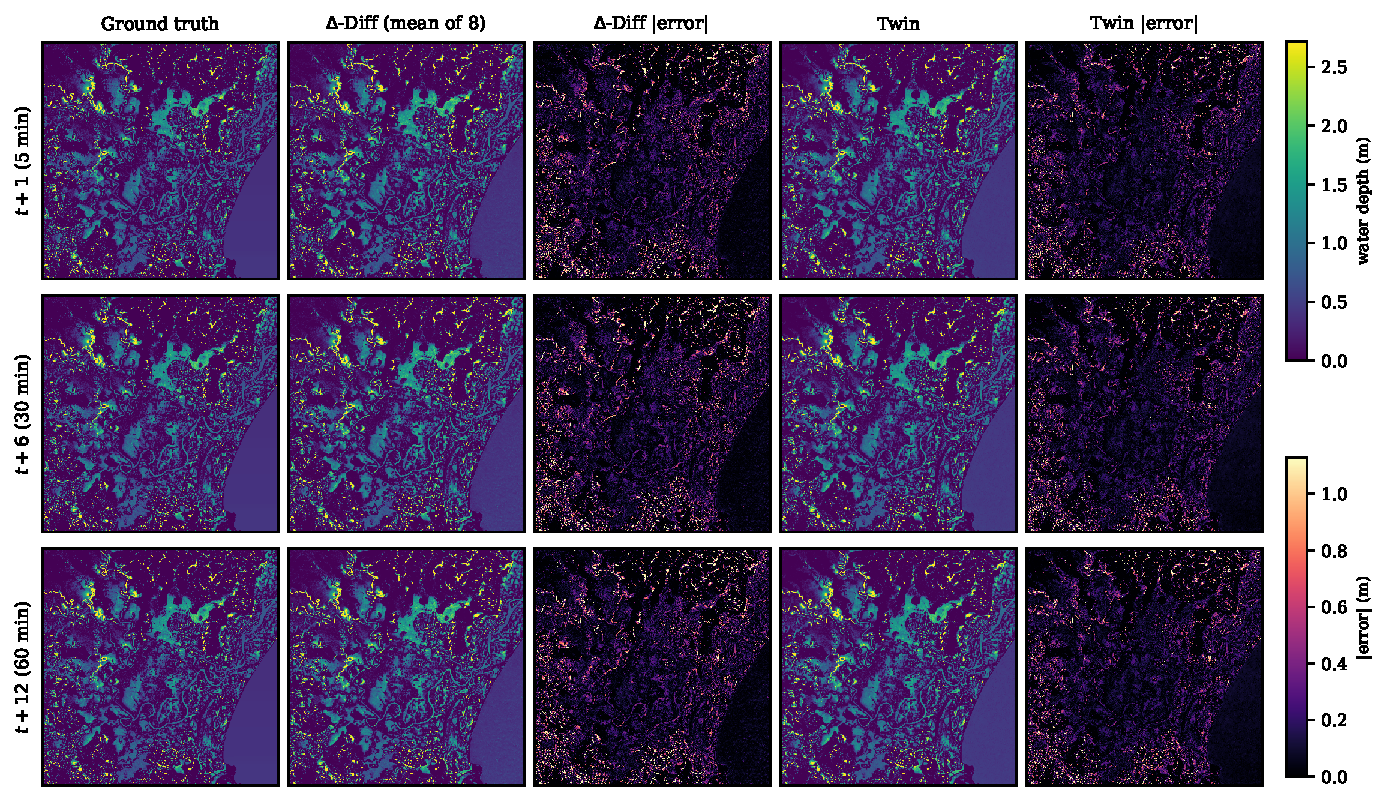
\includegraphics[width=0.72\linewidth]{figures/f7_qualitative_maps.pdf}
  \caption{Qualitative rollout at \mninetyfive{}, one representative test
  window (\ours{}: mean of 8 scenarios; \twin{}: single deterministic
  forecast; corrected checkpoints, \S\ref{sec:protocol}). Depth and error
  colormaps are each capped at the 99th percentile of ground truth (resp.\
  pooled error) to keep the flood extent and error texture visible against
  a small number of deep-channel outlier pixels. The error panels show a
  visible, not just numerical, difference: \twin{}'s error map is
  consistently darker (mean absolute error $\approx$0.105\,m across the
  three horizons shown, vs.\ $\approx$0.122\,m for \ours{}), concentrated
  similarly at flood-boundary pixels for both models. This single window
  is illustrative, not a substitute for the aggregate comparison below.}
  \label{fig:qualitative}
\end{figure}

The decision criteria were pre-registered before the comparison was run:
if \twin{} matches or beats the 8-scenario mean of \ours{} in every
regime, the generative mechanism adds nothing here; if \ours{} wins under
sparsity and ties or loses when dense, the generative premise is
confirmed where observation is incomplete; any mixed outcome is reported
per-regime with no blanket claim.

\begin{table}[H]
\centering
\caption{\ours{} (mean of 8 scenarios) vs.\ \twin{} (single deterministic
forecast), relative RMSE, mean $\pm$ std over 3 seeds (42/7/123), full
test protocol (13/13 windows) for all three regimes. \textbf{Bold} marks
the better model per row. The rightmost
column reports whether the per-seed difference (\ours{} $-$ \twin{}) has
a consistent sign across all 3 seeds --- our current significance check
(\S\ref{sec:protocol}).}
\label{tab:twinresults}
\begin{tabular}{lrrll}
\toprule
Regime & \ours{} & \twin{} & Winner & Consistent sign (3 seeds) \\
\midrule
dense & 0.001558 $\pm$ 0.000836 & $\mathbf{0.000417 \pm 0.000039}$ & \twin{}, $\times$3.7 & yes \\
\mfifty{} & $\mathbf{0.318425 \pm 0.043702}$ & 0.348852 $\pm$ 0.040779 & \ours{}, $\times$1.1 (weak) & \textbf{no} \\
\mninetyfive{} & 0.492443 $\pm$ 0.013940 & $\mathbf{0.344249 \pm 0.006248}$ & \twin{}, $\times$1.4 & yes \\
\bottomrule
\end{tabular}
\end{table}

The outcome is \textbf{mixed}, matching neither pre-registered blanket
claim: \twin{} dominates at the two extremes --- dense, where there is no
reconstruction ambiguity to resolve, and \mninetyfive{}, extreme sparsity,
where a naive prior would expect the generative model's advantage to be
\emph{largest} --- while \mfifty{} is genuinely undecided, with the sign
of the per-seed difference flipping between seeds. This non-monotone
pattern is, if anything, more informative than a clean win: it is not the
sparsity level itself that predicts a generative advantage, and a
tautological reading (``the target is deterministic, so of course the
deterministic model wins'') would predict uniform dominance --- which is
not what we observe. We return to what might explain the pattern in
\S\ref{sec:discussion}. As a robustness check, this qualitative pattern
(\twin{} wins at the extremes, \mfifty{} undecided) is unchanged from a
pre-correction read of the same comparison on the original checkpoints
($\times$3.55 dense, quasi-tie \mfifty{}, $\times$1.57 \mninetyfive{})
--- the convergence audit changed the exact numbers but not the
conclusion, which we read as evidence the verdict is not an artifact of
the correction itself. The verdict is also robust to the choice of
metric: at \mninetyfive{}, \twin{} leads on all six metrics we compute
(relative RMSE, NSE, CSI at both flood thresholds, the scenario-majority
median-mask CSI, and final-extent path IoU), while at \mfifty{} \emph{no}
metric shows a seed-consistent direction --- the undecided call at
\mfifty{} is not an artifact of reporting relative RMSE.
\FloatBarrier

\subsection{Cross-regional transfer, zero-shot}
\label{sec:zeroshot}
FloodCastBench's authors also evaluate FNO+ under zero-shot cross-regional
transfer: weights trained on one event, frozen, and evaluated on another.
We replicate this protocol exactly --- Australia-trained checkpoints,
frozen weights \emph{and} frozen normalization, evaluated on the UK 2015
event --- for both models and all three seeds
(Table~\ref{tab:zeroshot}).

\begin{table}[H]
\centering
\caption{Zero-shot cross-regional transfer (Australia $\to$ UK, 60\,m,
dense observation), relative RMSE against the benchmark's published FNO+
transfer result under the same frozen-weights protocol. \twin{} is
single-pass deterministic output, matching FNO+'s output type; \ours{} is
its 8-scenario mean. Mean $\pm$ std over the same 3 Australia-trained
seeds as everywhere else in this paper.}
\label{tab:zeroshot}
\begin{tabular}{lrr}
\toprule
Model & relRMSE (zero-shot UK) $\downarrow$ & vs.\ FNO+ published \\
\midrule
FNO+ \citep{floodcastbench2025} & 0.024771 & --- \\
\ours{} (3 seeds)  & 0.001850 $\pm$ 0.000498 & $\sim$13$\times$ better \\
\twin{} (3 seeds)  & $\mathbf{0.000664 \pm 0.000019}$ & $\sim$\textbf{37$\times$ better} \\
\bottomrule
\end{tabular}
\end{table}

Both models transfer dramatically better than the published baseline, the
twin ahead of the diffusion model --- the in-domain ordering survives the
domain shift untouched, with remarkably low seed variance for the twin.
Two honest qualifications keep this from being a headline claim yet.
First, the UK test split supports only \textbf{3 evaluation windows} ---
the direction is consistent across seeds and across both models, but a
ratio computed on 3 windows is a strong signal, not a settled number.
Second, we have verified our transfer protocol matches the published
description (frozen weights, adjusted target domain), but the
publication does not specify whether its normalization statistics were
also frozen from the source domain as ours are; if that choice differed,
the comparison is between closely related but not identical protocols.

\blocked{The consolidation experiment is the same probe on the
benchmark's \emph{other} published transfer pair, Pakistan $\to$
Mozambique (480\,m, low-fidelity; published FNO+ transfer relRMSE
0.078633), whose test split supports $\sim$20 evaluation windows ---
enough to retire the small-sample caveat. It requires first training the
twin in-domain on Pakistan (no Pakistan checkpoint previously existed);
that training was launched, ran cleanly to epoch $\sim$24 of 300
($\sim$26\,min/epoch on the $810\times441$ grid), and is currently
\textbf{paused} --- the shared GPU was reclaimed --- to be resumed when
compute frees. Outcome contract: if the Pakistan$\to$Mozambique ordering
matches Table~\ref{tab:zeroshot}, the transfer section graduates to a
headline claim with the UK result as supporting evidence; if it
contradicts it, both results are reported and the section is reframed
around when transfer holds.}

\subsection{Structured sensor layouts vs.\ random masks}
\label{sec:masks}
Training uses i.i.d.\ random observation masks; real sensor networks are
not i.i.d. We evaluate two structured mask families never seen in
training, at matched sensor budget (Table~\ref{tab:masks}).

\begin{table}[H]
\centering
\caption{\ours{} relative RMSE under structured vs.\ random evaluation
masks at matched sensor budget (seed 42; the cluster/\mfifty{} result was
confirmed on a second seed: 0.597 vs.\ 0.609).}
\label{tab:masks}
\begin{tabular}{lrrl}
\toprule
Mask & \mfifty & \mninetyfive & vs.\ random \\
\midrule
Random (training distribution) & 0.395 & 0.567 & --- \\
Gauge (spatially distributed)  & 0.393 & 0.585 & $\approx$ identical \\
Cluster (contiguous gap)       & 0.609 & 0.706 & \textbf{+54\% / +25\%} \\
\bottomrule
\end{tabular}
\end{table}

The \textbf{gauge} mask --- structured, but still spatially distributed
--- transfers almost perfectly. The \textbf{cluster} mask leaves a large
contiguous region entirely unobserved, a spatial regime never encountered
during training, and degrades markedly. This is a real, physically
interpretable generalization boundary: the model's implicit assumption is
\emph{distributed} partial observation, not merely a sensor \emph{count}
--- a deployment limitation worth stating plainly.

\subsection{Calibration}
\label{sec:calibration}
\begin{figure}[H]
  \centering
  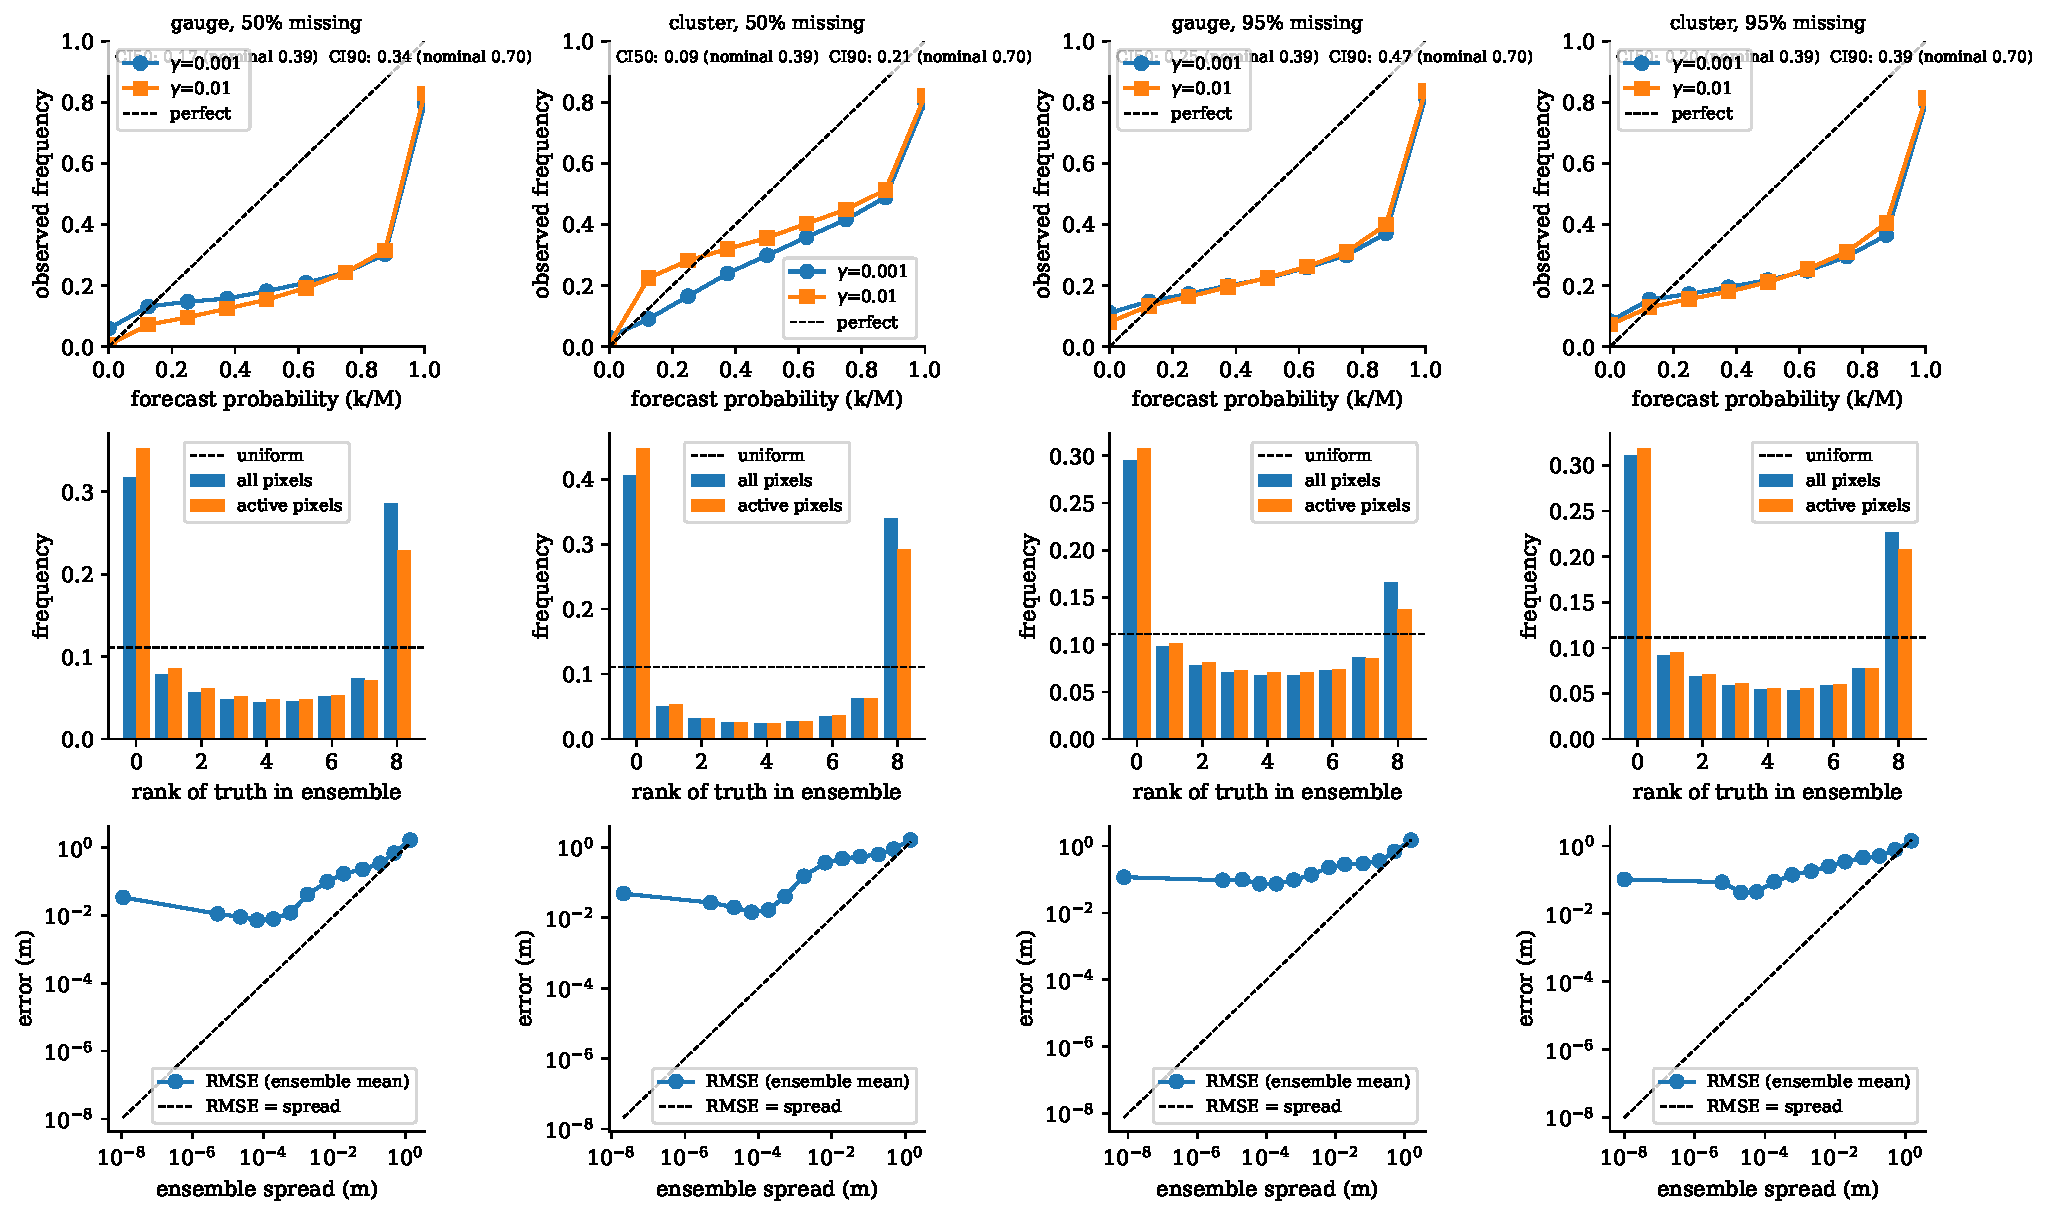
\includegraphics[width=0.9\linewidth]{figures/f5_calibration_diagnostics.pdf}
  \caption{Calibration diagnostics for \ours{} across the four structured-mask
  $\times$ sparsity conditions (columns). Rows: reliability of the
  scenario-fraction wet/dry forecast at two flood thresholds; rank of the
  truth within the 8-member ensemble (a U shape indicates overconfidence);
  ensemble spread vs.\ actual error of the ensemble mean. Under-coverage
  is systematic in every condition; sparsity level, not mask structure,
  dominates calibration quality.}
  \label{fig:calibration}
\end{figure}

\ours{}'s 8-scenario ensembles show \textbf{severe, systematic
under-coverage} across all tested conditions
(Figure~\ref{fig:calibration}): a nominal 90\% central interval
(finite-ensemble corrected) covers only 20--47\% of true outcomes
depending on sparsity and mask structure. Sparsity level, not mask
structure, dominates calibration quality --- counter-intuitively,
\mninetyfive{} is better calibrated than \mfifty{} for both mask families.

\paragraph{Is a generative model even needed for uncertainty?}
The natural rejoinder --- ``a deterministic model cannot quantify
uncertainty'' --- is false as stated: a \emph{deep ensemble} of
independently trained deterministic models
\citep{lakshminarayanan2017deep} is the standard baseline, and our three
\twin{} seeds provide one at zero additional training cost.
Figure~\ref{fig:calibcomp} makes the comparison at both sparsities, with
the twin ensemble evaluated on the same random masks used everywhere else
in this paper and \ours{} on its closest matched condition (random masks
at \mfifty{}; the structured gauge/cluster masks at \mninetyfive{}, since
no random-mask calibration run was performed at that sparsity). The result
is symmetric and sobering at both sparsities: at \mfifty{}, the twin
ensemble ($M{=}3$) covers 47\% of its corrected 50\%-interval nominal
(\ours{}, $M{=}8$, random masks: 40\%); at \mninetyfive{}, the twin
ensemble covers 70\% (\ours{}: 64\% gauge, 52\% cluster). \textbf{At no
sparsity tested is the twin ensemble less well calibrated than the
diffusion ensemble} --- if anything the reverse holds slightly, and the
rank histograms show the diffusion ensemble is, if anything, more
overconfident in shape. On this benchmark, calibration as measured so far
does not supply the generative model's missing justification: the
uncertainty-based defense of diffusion is not merely unproven, it is
actively contradicted by the one standard baseline it should be compared
against.

\begin{figure}[H]
  \centering
  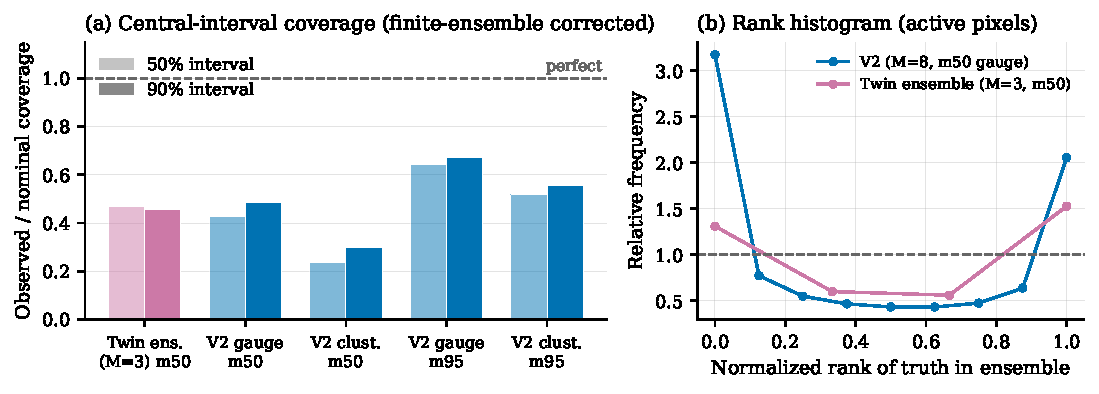
\includegraphics[width=\linewidth]{figures/f6_calibration_comparison.pdf}
  \caption{Uncertainty quality: \ours{} diffusion ensembles vs.\ a deep
  ensemble of deterministic twins, at both tested sparsities. (a) Observed
  over nominal coverage (finite-ensemble corrected; 1.0 = perfectly
  calibrated) --- every condition is severely under-covered, and the twin
  ensemble is never worse than \ours{}. (b) Rank histograms over active
  pixels at \mfifty{} (matched random masks): both are U-shaped
  (overconfident), \ours{} more strongly so. Caveat: at \mninetyfive{},
  \ours{} is evaluated on structured masks (no random-mask run at that
  sparsity) while the twin ensemble uses random masks --- \S\ref{sec:masks}
  showed the gauge mask behaves like random, so this likely understates
  rather than overstates \ours{}'s calibration there.}
  \label{fig:calibcomp}
\end{figure}

\blocked{Remaining for this subsection: a matched random-mask \ours{}
evaluation at \mninetyfive{} (to remove the one remaining mask-type
caveat), and a sharpness-aware score (CRPS) to complement pure coverage.}

\subsection{Ablations and cost}
\label{sec:ablations}
\blocked{Two studies are planned but not yet run: (i) a component
ablation of \ours{} (delta parametrization, target-step rainfall, spatial
encoder, change-weighted loss, rollout-aware training, number of diffusion
steps); (ii) a cost table --- parameters, inference latency, peak memory,
training wall-clock --- pricing, with measured numbers rather than the
architectural 320$\times$ count, the fact that one \ours{} prediction
costs 40 denoising steps $\times$ 8 scenarios against the twin's single
forward pass. The cross-event transfer study formerly listed here has
graduated to \S\ref{sec:zeroshot}.}

% ============================================================
\section{Discussion}
\label{sec:discussion}

\paragraph{When does generative forecasting pay off here?} Not uniformly,
and not where a naive prior would place it. \twin{} wins decisively in two
regimes that sit at opposite ends of the observability spectrum: dense,
where the state is fully known and there is no reconstruction ambiguity
for a generative model to resolve, and \mninetyfive{}, extreme sparsity,
where --- if the field's calibration-pivot intuition were correct ---
scenario diversity should matter \emph{most}. \ours{} does not lose at
\mninetyfive{}; it loses by a similar margin to how \twin{} loses at
\mfifty{}, and \mfifty{} itself is the one regime our data cannot call.
The honest summary is that \emph{sparsity level alone does not predict
the generative model's relative advantage} on this benchmark, which is a
sharper and less convenient finding than either pre-registered blanket
claim we set out to test.

\paragraph{Where the gains actually come from.} The attribution question
--- what, in this line of work, produces the reported improvements? ---
has a measurable answer here. The three-orders-of-magnitude jump from
\absdiff{} to \ours{} comes from the delta-space target and regime-aware
scale (\S\ref{sec:paramresults}); it survives removing the extra context
(\S\ref{sec:vsfnoplus}); and it transfers \emph{in full} to the
deterministic twin, which then goes further. Nothing in our measurements
requires the generative mechanism to explain any of the gains --- and the
mechanism itself, compared under matched everything, never shows a
seed-consistent advantage in any regime. On this benchmark, the
architecture and parametrization are the contribution; the sampler is a
cost.

\paragraph{A tentative mechanistic reading.} \S\ref{sec:mechanism}
established that the scale of \ours{}'s target ($\sigma_\Delta$ at
observed pixels vs.\ closer to $\sigma_{\text{field}}$ at masked ones,
\S\ref{sec:regime}) governs how hard the generative task is. The same
compression appears in a different comparison: \S\ref{sec:paramresults}
showed the \absdiff{}-vs-\ours{} gap shrinking sharply from dense to
\mninetyfive{} ($970\times \to 1.9\times$) as the masked-pixel target
scale grows toward the field scale. If an analogous effect operates on
the \twin{}-vs-\ours{} margin --- the effective reconstruction task
getting \emph{harder} for both models as sparsity increases, but in a way
that compresses whatever residual generative benefit exists faster than
it compresses \twin{}'s deterministic estimate --- it would predict
exactly the observed non-monotonicity: a wide \twin{} margin at both ends
of the spectrum and a narrow, noisy one in between. We flag this as a
hypothesis consistent with, but not established by, the current data;
distinguishing it from ordinary seed variance at \mfifty{} needs the
additional seeds noted below.

\paragraph{Epistemic vs.\ aleatoric, and what diffusion was imported for.}
Generative forecasting earned its place in domains with genuine
trajectory-level stochasticity --- medium-range weather beyond the
deterministic predictability horizon, where an ensemble of futures is the
\emph{correct} object to predict \citep{gencast2024}. FloodCastBench's
ground truth is a single deterministic simulation: at short horizons
there is one future, and the only uncertainty partial observation
introduces is epistemic --- reconstruction ambiguity, which shrinks with
information rather than growing with lead time. Our results are what one
would expect if that distinction matters: the generative machinery,
imported into a regime whose premise it does not satisfy, prices in
scenario diversity that the task does not reward
(\S\ref{sec:calibration} shows even its uncertainty estimates are no
better than a deep ensemble's). We state this as an interpretive frame
rather than a demonstrated law; the noise-free-vs-noisy contrast of
\citet{spatiallyawarediffusion2024} suggests the boundary shifts once
observations themselves carry noise, which our benchmark's synthetic
sensors do not.

\paragraph{Deployment implications of the cluster-mask result
(\S\ref{sec:masks}).} The generalization failure under contiguous
coverage gaps is a deployment-relevant, physically interpretable limit:
\ours{} implicitly assumes distributed partial observation, not merely a
fixed sensor count. A network with a large unmonitored region should not
expect out-of-the-box performance matching a distributed network of equal
size, for either model in this comparison.

\paragraph{Is the twin an FNO replacement? A scoped answer.} The twin
beats FNO+ in-domain ($\sim$9.4$\times$) and in zero-shot transfer
($\sim$37$\times$, with the caveats of \S\ref{sec:zeroshot}) --- it is
natural to ask whether it should simply replace Fourier neural operators
for this problem class. We answer deliberately narrowly. The inductive
bias that favors the twin here --- local multi-scale convolution and
attention, well suited to sharp, localized wetting fronts under sparse
observation --- is the same bias that predicts it should \emph{lose} on
the globally smooth fields FNO was designed and validated on
(Navier--Stokes, Darcy flow), where spectral mixing and
resolution-invariance are genuine advantages \citep{li2021fno}. No
architecture dominates across problem classes, and a claim of universal
superiority would be refuted by testing on FNO's home terrain --- a test
we consider the right \emph{future} adversarial experiment, not a gap in
this paper's claims. What our results support is the scoped statement:
for sparse-observation forecasting of sharp-fronted flood fields, the
twin's design point is preferable to FNO+ on every axis we measured.
Two confounds remain before even that scoped claim is fully clean: the
twin differs from FNO+ in \emph{both} backbone and parametrization, and
attributing its margin between the two requires giving FNO+ the same
delta-space, regime-aware target --- an experiment using the same
training infrastructure as our FNO+ reproduction, planned as the
decisive next step on this axis.

\paragraph{Was it worth it?} Any residual generative advantage --- real
at \mninetyfive{} within our data, unresolved at \mfifty{} --- must still
be weighed against \ours{}'s measured cost over \twin{}: 40 denoising
steps $\times$ 8 scenarios per prediction against a single forward pass
(\S\ref{sec:ablations}). We do not yet have that price attached to a
measured number (cost table pending), so we do not adjudicate the trade
here.

\paragraph{A procedural corollary.} Everything above was only visible
because a parameter-matched deterministic twin existed. The twin cost a
configuration change --- not a new model, not a new codebase --- and it
converted ``our diffusion model beats the baseline'' into ``our
representation choices beat the baseline; the sampler subtracts value.''
We suggest the field adopt the practice, stated modestly: \emph{before
attributing a forecasting gain to a generative mechanism, evaluate the
same network with the mechanism switched off}. A single rigorous
demonstration that the control can reverse a paper's headline attribution
--- which is what this paper documents --- is, we think, sufficient
motivation; it does not require our substantive findings to generalize
beyond this benchmark, and we make no such claim
(\S\ref{sec:limitations}).

\subsection{Limitations}
\label{sec:limitations}
\begin{itemize}
  \item Ground truth is a single deterministic hydraulic simulation per
    event (\S\ref{sec:calibmeaning}) --- calibration claims are scoped to
    reconstruction ambiguity, not physical aleatoric uncertainty.
  \item Sparsity is synthetic: random masks plus two structured families.
    Real sensor-network geometries may differ in ways the cluster result
    (\S\ref{sec:masks}) only partially anticipates. Likewise the
    benchmark's sensors are noise-free --- the regime
    \citet{spatiallyawarediffusion2024} identify as maximally favorable
    to deterministic models; an observation-noise axis is a natural
    extension we have deliberately not priced into this paper's claims.
  \item All in-domain results concern a single flood event (Australia).
    The zero-shot transfer study (\S\ref{sec:zeroshot}) is evidence of
    cross-event robustness but rests on a 3-window UK test split and one
    unverifiable protocol detail (whether the published transfer numbers
    froze source-domain normalization as ours do); the in-domain UK study
    and the Pakistan$\to$Mozambique probe are both pending.
  \item The central-comparison significance check (Table~\ref{tab:twinresults})
    is a seed-paired sign test ($n{=}3$, one difference per seed) rather
    than the pre-registered window$\times$seed paired test ($n{=}39$):
    the evaluator currently logs only the aggregate relative RMSE per
    run, not a per-window breakdown. This is sufficient to establish a
    consistent-vs-inconsistent sign but not a calibrated $p$-value; adding
    per-window logging before any future re-evaluation is planned
    (\S\ref{sec:protocol}).
  \item The \mfifty{} regime's undecided verdict is based on 3 seeds
    with a sign flip; distinguishing a genuine near-tie from insufficient
    seed count is not yet possible with this sample size.
  \item \textbf{Scope of the generalization claim.} Even once extended to
    all four FloodCastBench events, these are draws from a single
    benchmark's data-generation pipeline --- the same hydraulic simulator,
    the same curation choices --- not independent replications across
    simulators or institutions. A pattern that holds across all four could
    still be a property of this simulator (e.g.\ its numerical damping)
    rather than of flood dynamics in general. Likewise, testing the
    matched-twin protocol on 1--2 additional generative architectures
    rules out ``artifact of one architecture'' but falls far short of
    covering the space of generative model designs. We therefore separate
    two claims of different strength: the \emph{procedural}
    recommendation --- that any claimed generative advantage in this
    class of problem should be checked against a parameter-matched
    deterministic twin --- is supported by demonstrating the check
    matters even once; the \emph{substantive} finding --- the specific
    mixed pattern we measure --- is scoped to FloodCastBench and the
    architectures tested, and should not be read as a general claim
    about generative spatiotemporal forecasting.
\end{itemize}

% ============================================================
\section*{Reproducibility Statement}
Code, configurations, and seeds for every reported run are version
controlled. All headline comparisons use $\geq 3$ seeds; no single-seed
number appears without an explicit label. Every model comparison holds
input context and evaluation protocol fixed, and any remaining asymmetry
is stated next to the number it affects. Each sparsity regime is
smoke-tested before full training --- a discipline adopted after a live
incident in which an unguarded normalization term produced non-finite
training losses under the sparse regime specifically, caught and fixed the
same day. The statistical bias specific to deterministic-vs-generative
comparisons (\S\ref{sec:twin}) is documented as a permanent methodological
rule after being caught on this project's own internal metrics.
\blocked{Repository URL will be added when the draft is frozen.}

% ============================================================
\bibliographystyle{plainnat}
\bibliography{refs}

\end{document}
